\section{Qgis}
\begin{frame}
    \begin{figure}
        \centering
        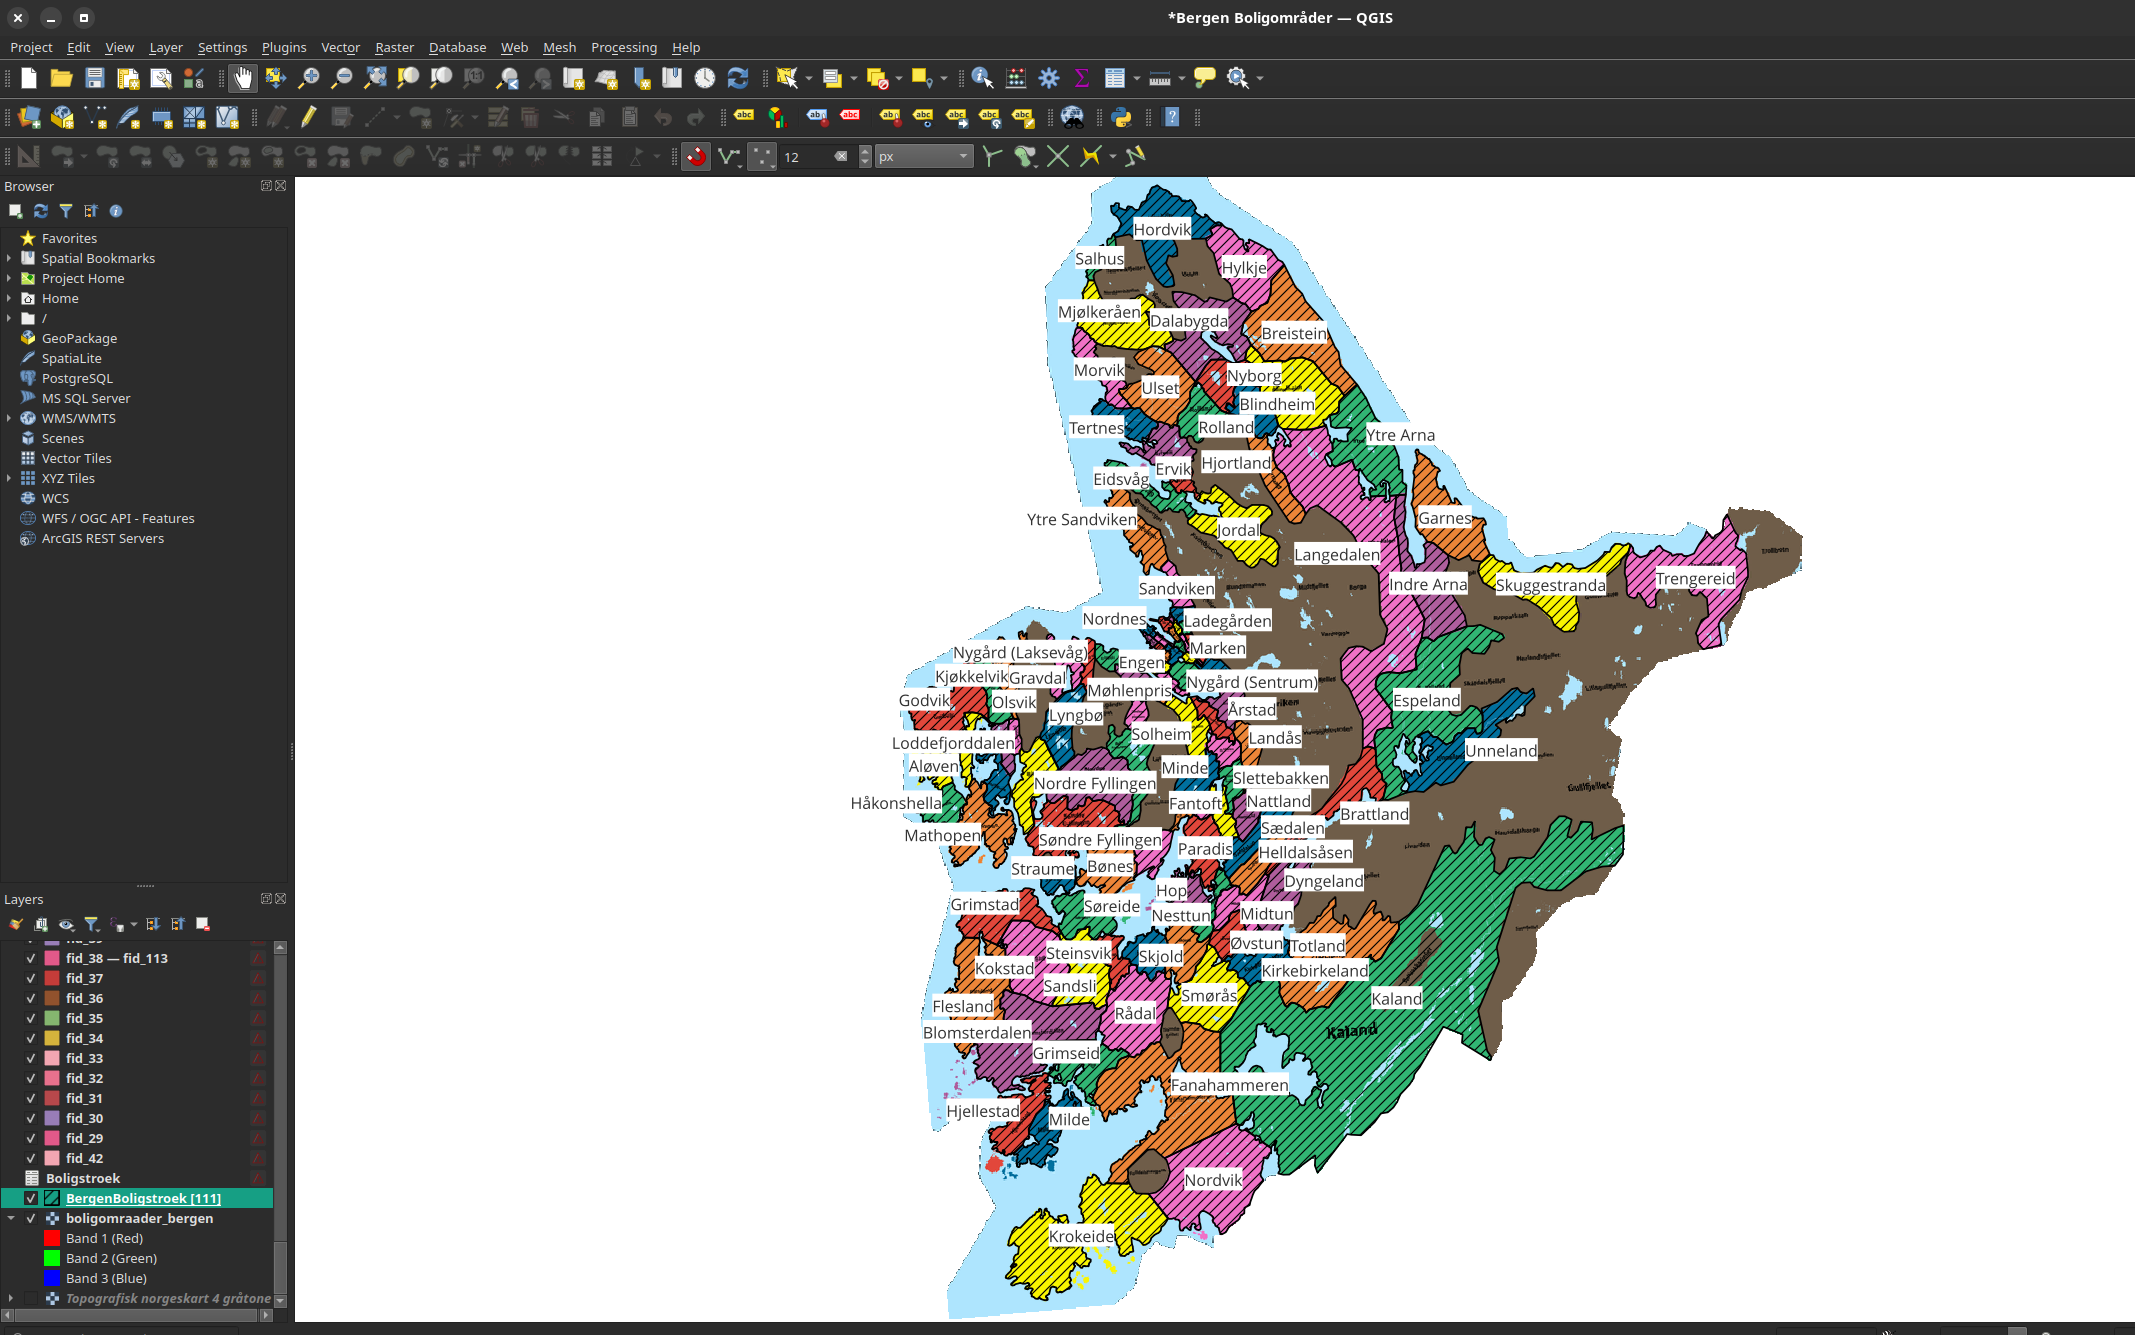
\includegraphics[height = 6cm]{images/qgisOverview.png}%
        \caption{Qgis - A programme of horror}
    \end{figure}
\end{frame}

\begin{frame}
    \begin{figure}
        \centering
        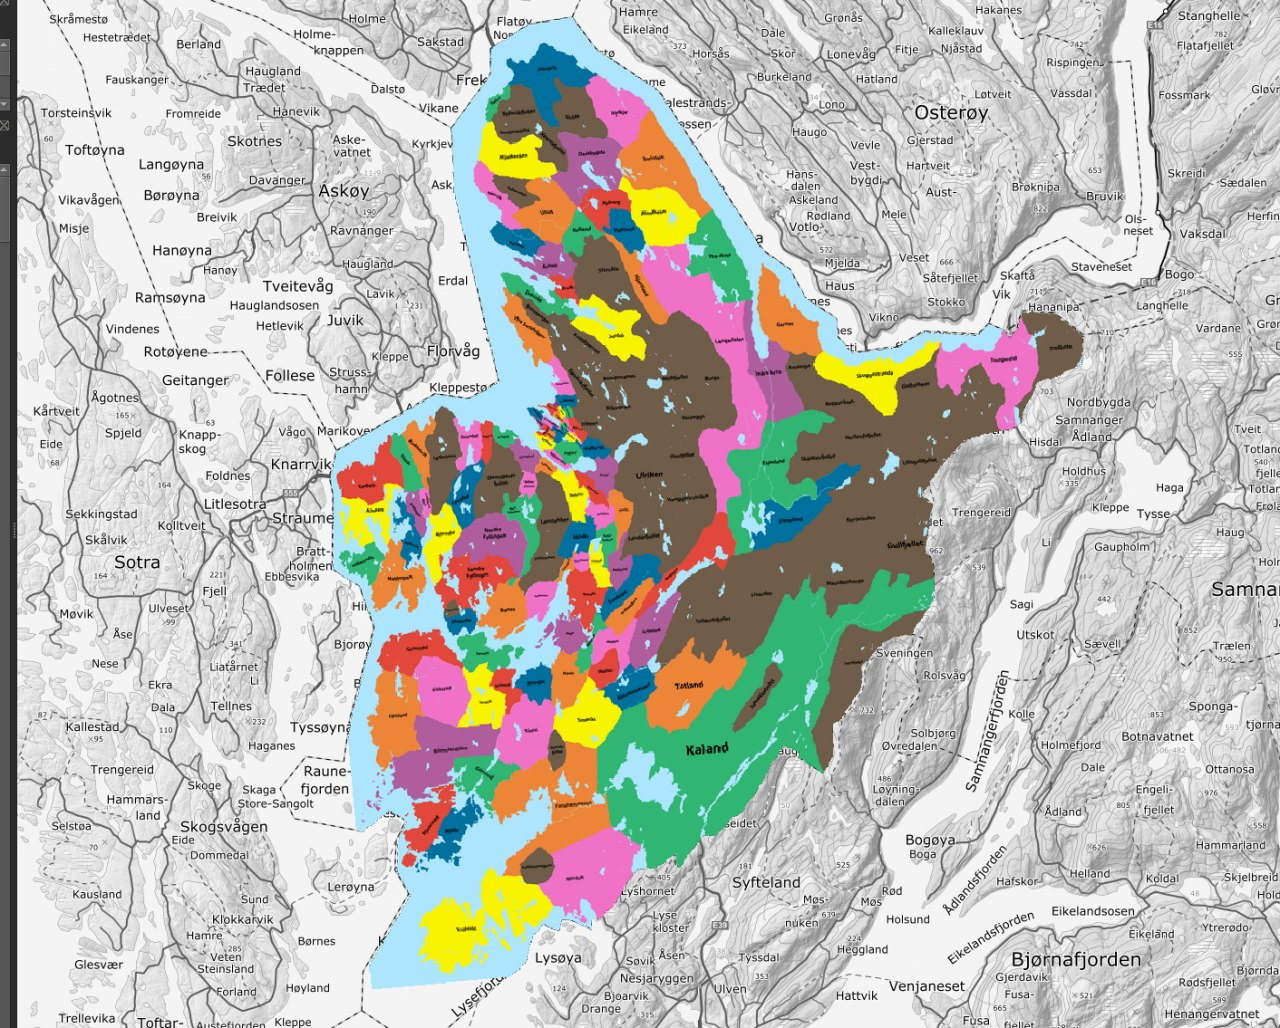
\includegraphics[height = 6cm]{images/qgis1.jpg}%
        \caption{Initialiser korrekte layers}
    \end{figure}
\end{frame}

\begin{frame}
    \begin{figure}
        \centering
        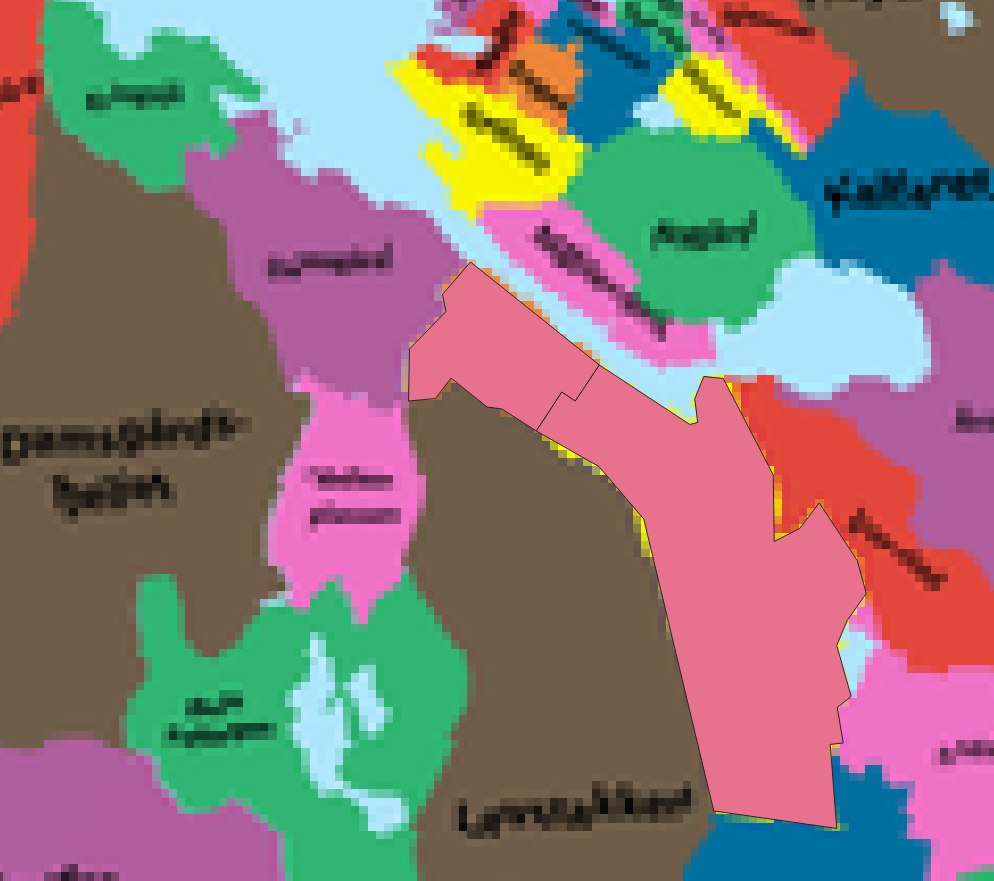
\includegraphics[height = 6cm]{images/qgis2.png}%
        \caption{Tegning}
    \end{figure}
\end{frame}

\begin{frame}
    \begin{figure}
        \centering
        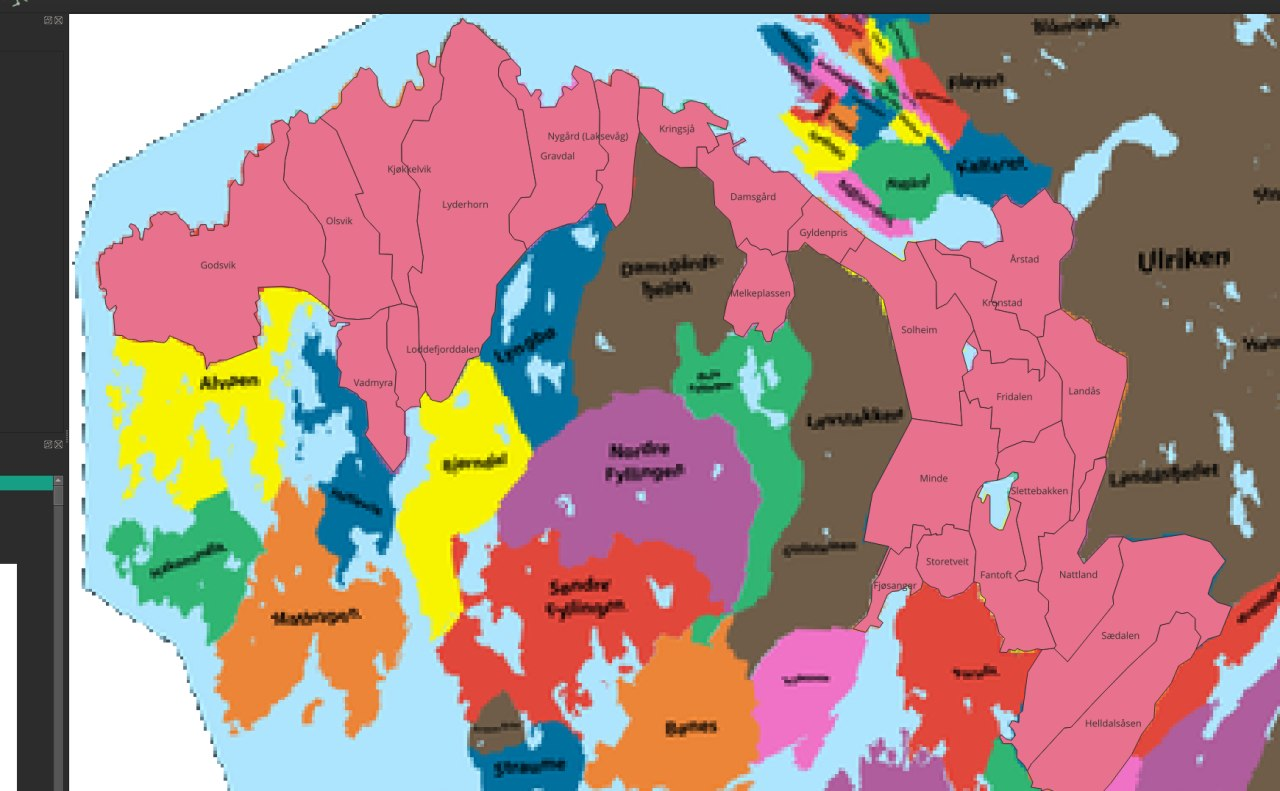
\includegraphics[height = 6cm]{images/qgis3.jpg}%
        \caption{Mer tegning}
    \end{figure}
\end{frame}

\begin{frame}
    \begin{figure}
        \centering
        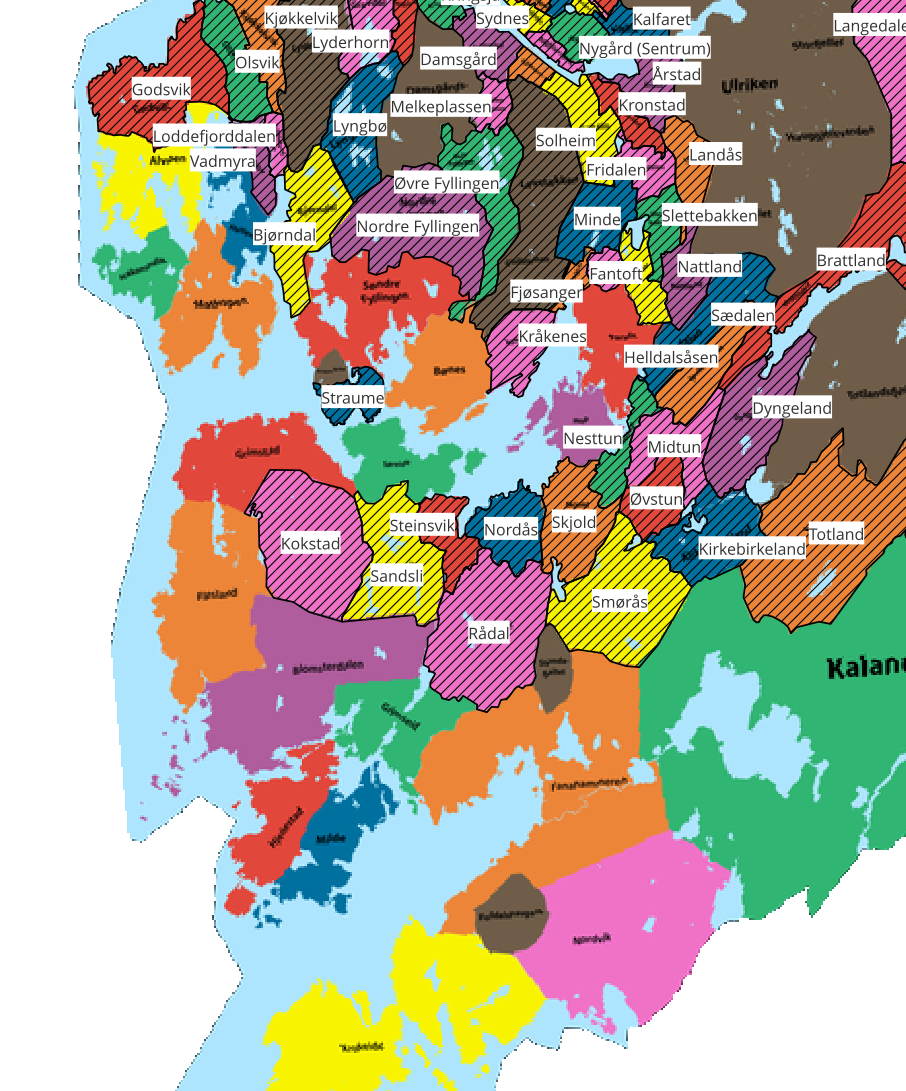
\includegraphics[height = 6cm]{images/qgis4.png}%
        \caption{Enda mer tegning}
    \end{figure}
\end{frame}

\begin{frame}
    \begin{figure}
        \centering
        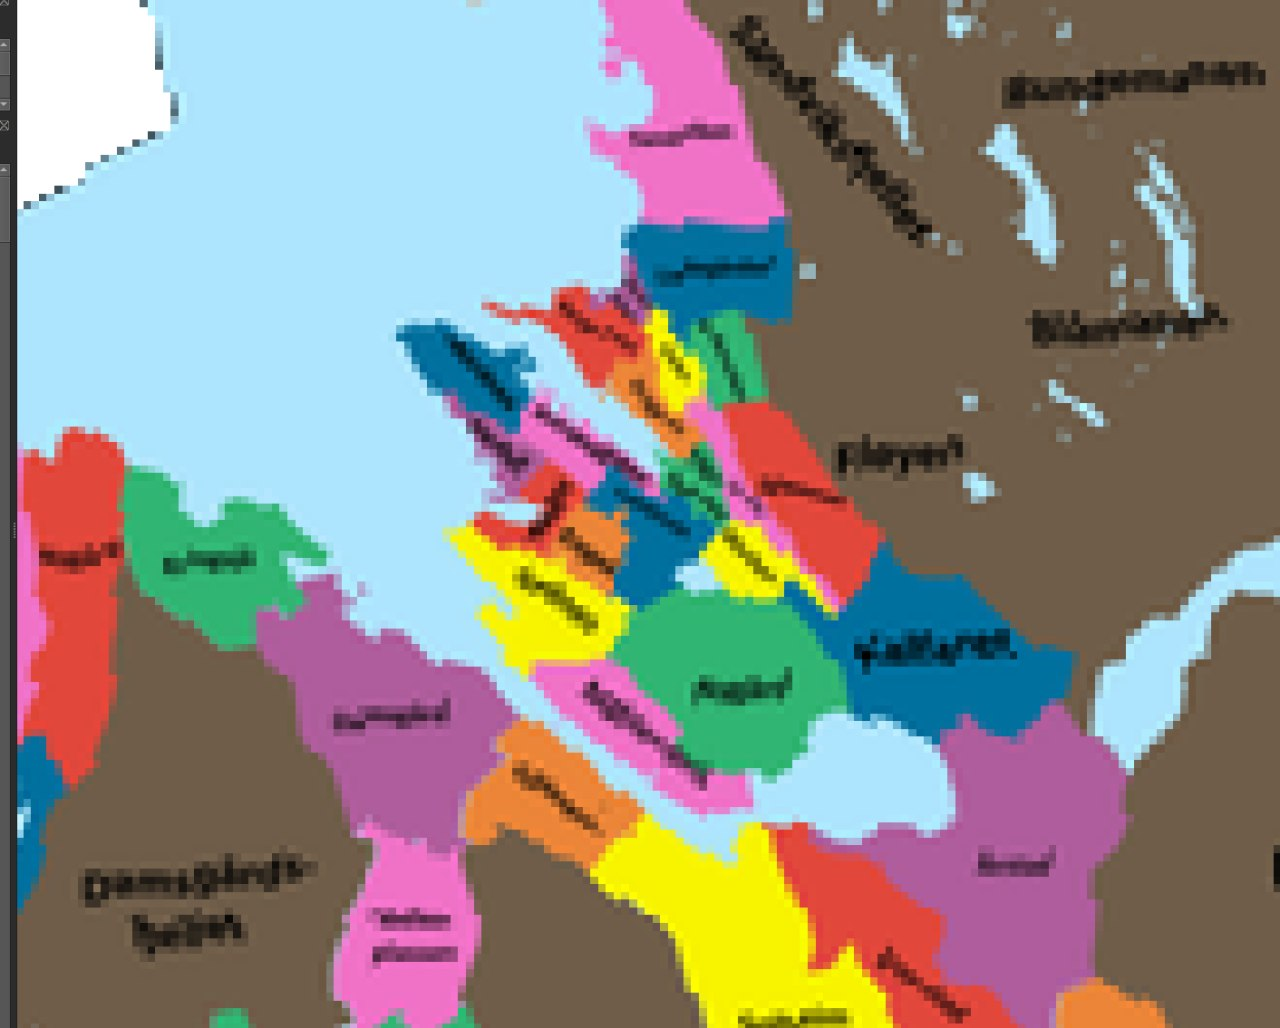
\includegraphics[height = 6cm]{images/qgis5.png}%
        \caption{Sentrum???}
    \end{figure}
\end{frame}

\begin{frame}
    \begin{figure}
        \centering
        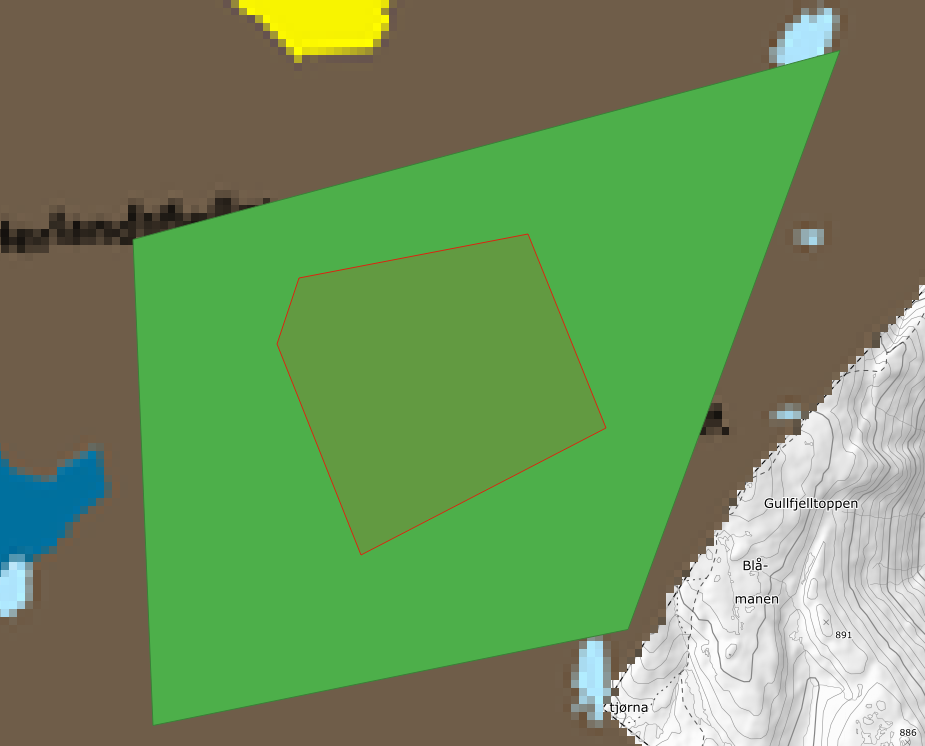
\includegraphics[height = 6cm]{images/qgis_shapeInShape.png}%
        \caption{Innsjøer?}
    \end{figure}
\end{frame}

\begin{frame}
    \begin{figure}
        \centering
        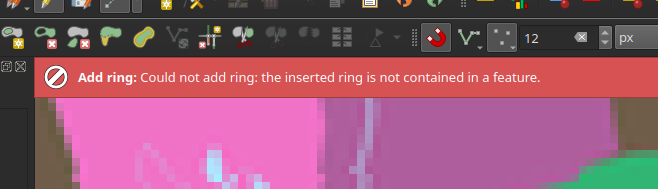
\includegraphics[height = 4cm]{images/qgis_ringInRing.png}%
        \caption{Er EPSG:25832 det man ser?}
    \end{figure}
\end{frame}

\begin{frame}
    \begin{figure}
        \centering
        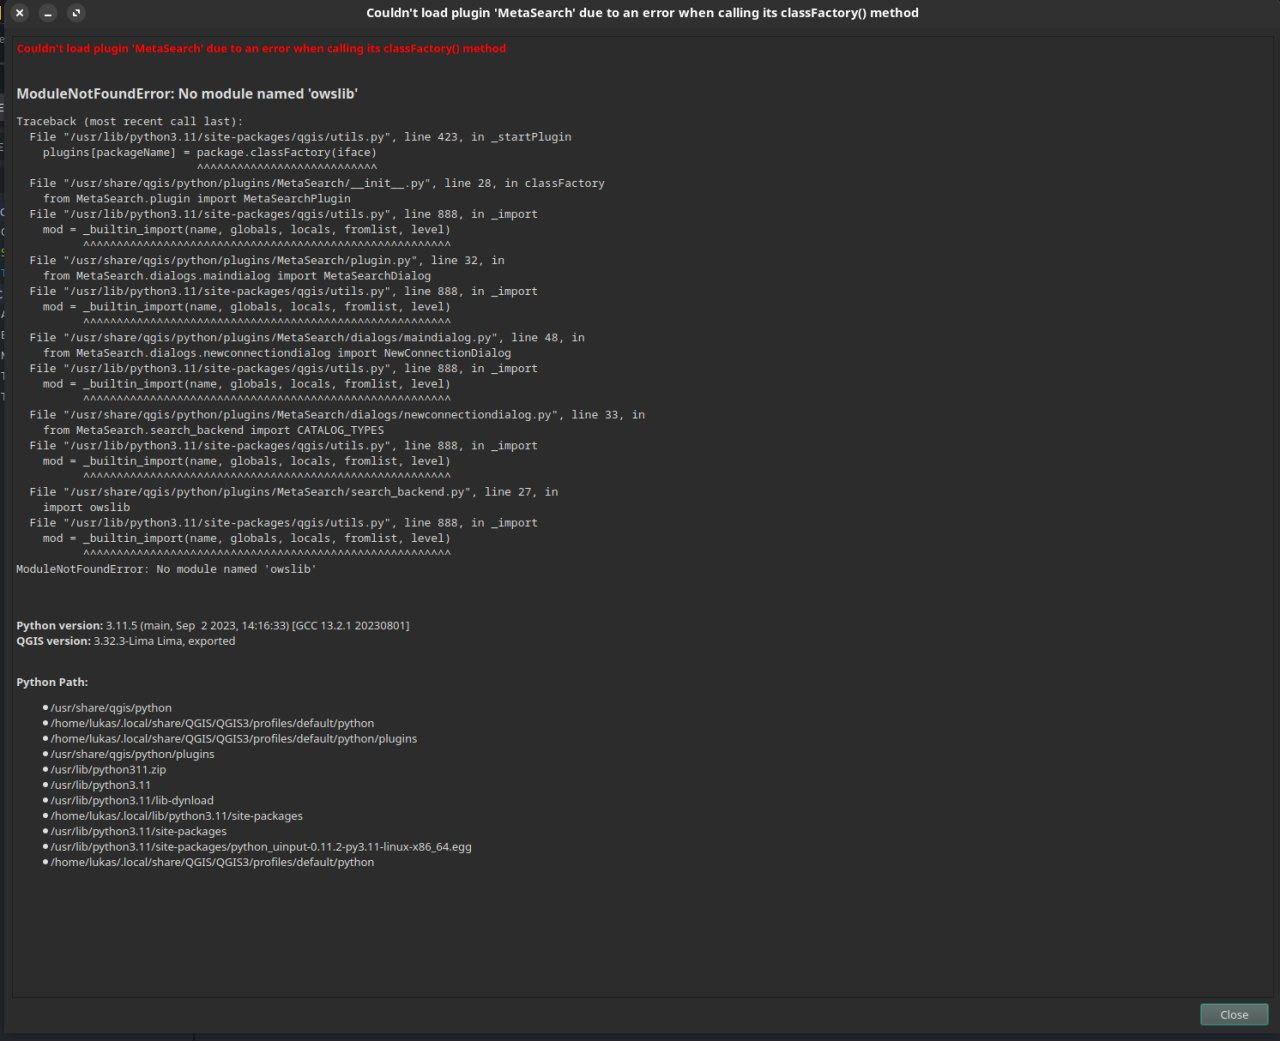
\includegraphics[height = 6cm]{images/qgis_pythonerror.jpg}%
        \caption{Python-Error}
    \end{figure}
\end{frame}

\begin{frame}
    \begin{figure}
        \centering
        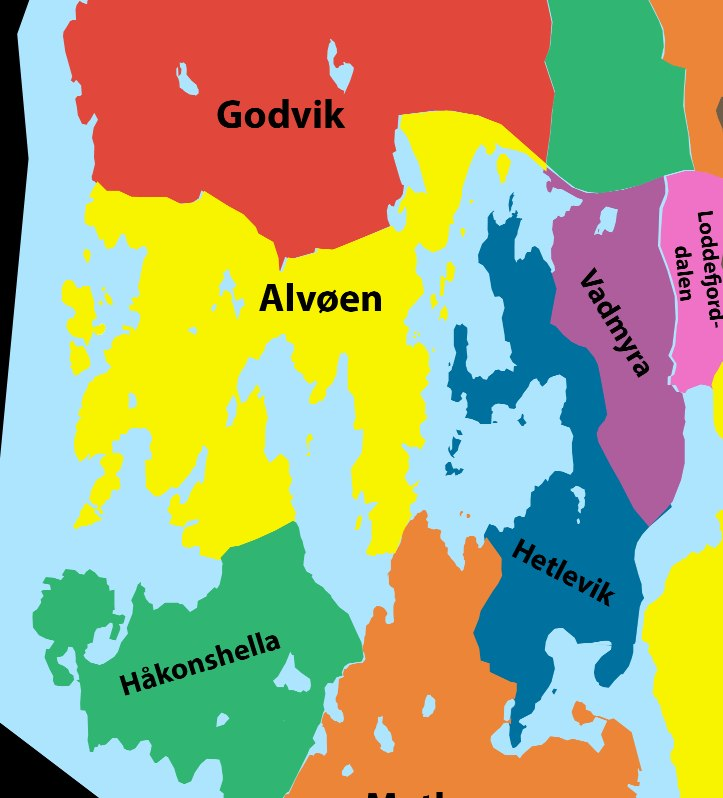
\includegraphics[height = 6cm]{images/qgis_islands.jpg}%
        \caption{Øyer?}
    \end{figure}
\end{frame}

\begin{frame}
    \begin{alertblock}{Error}
        \enquote{Could not add multi part element. This layer (type multilayer) does not support multi layer elements.}
    \end{alertblock}
%    \begin{figure}
%        \centering
%        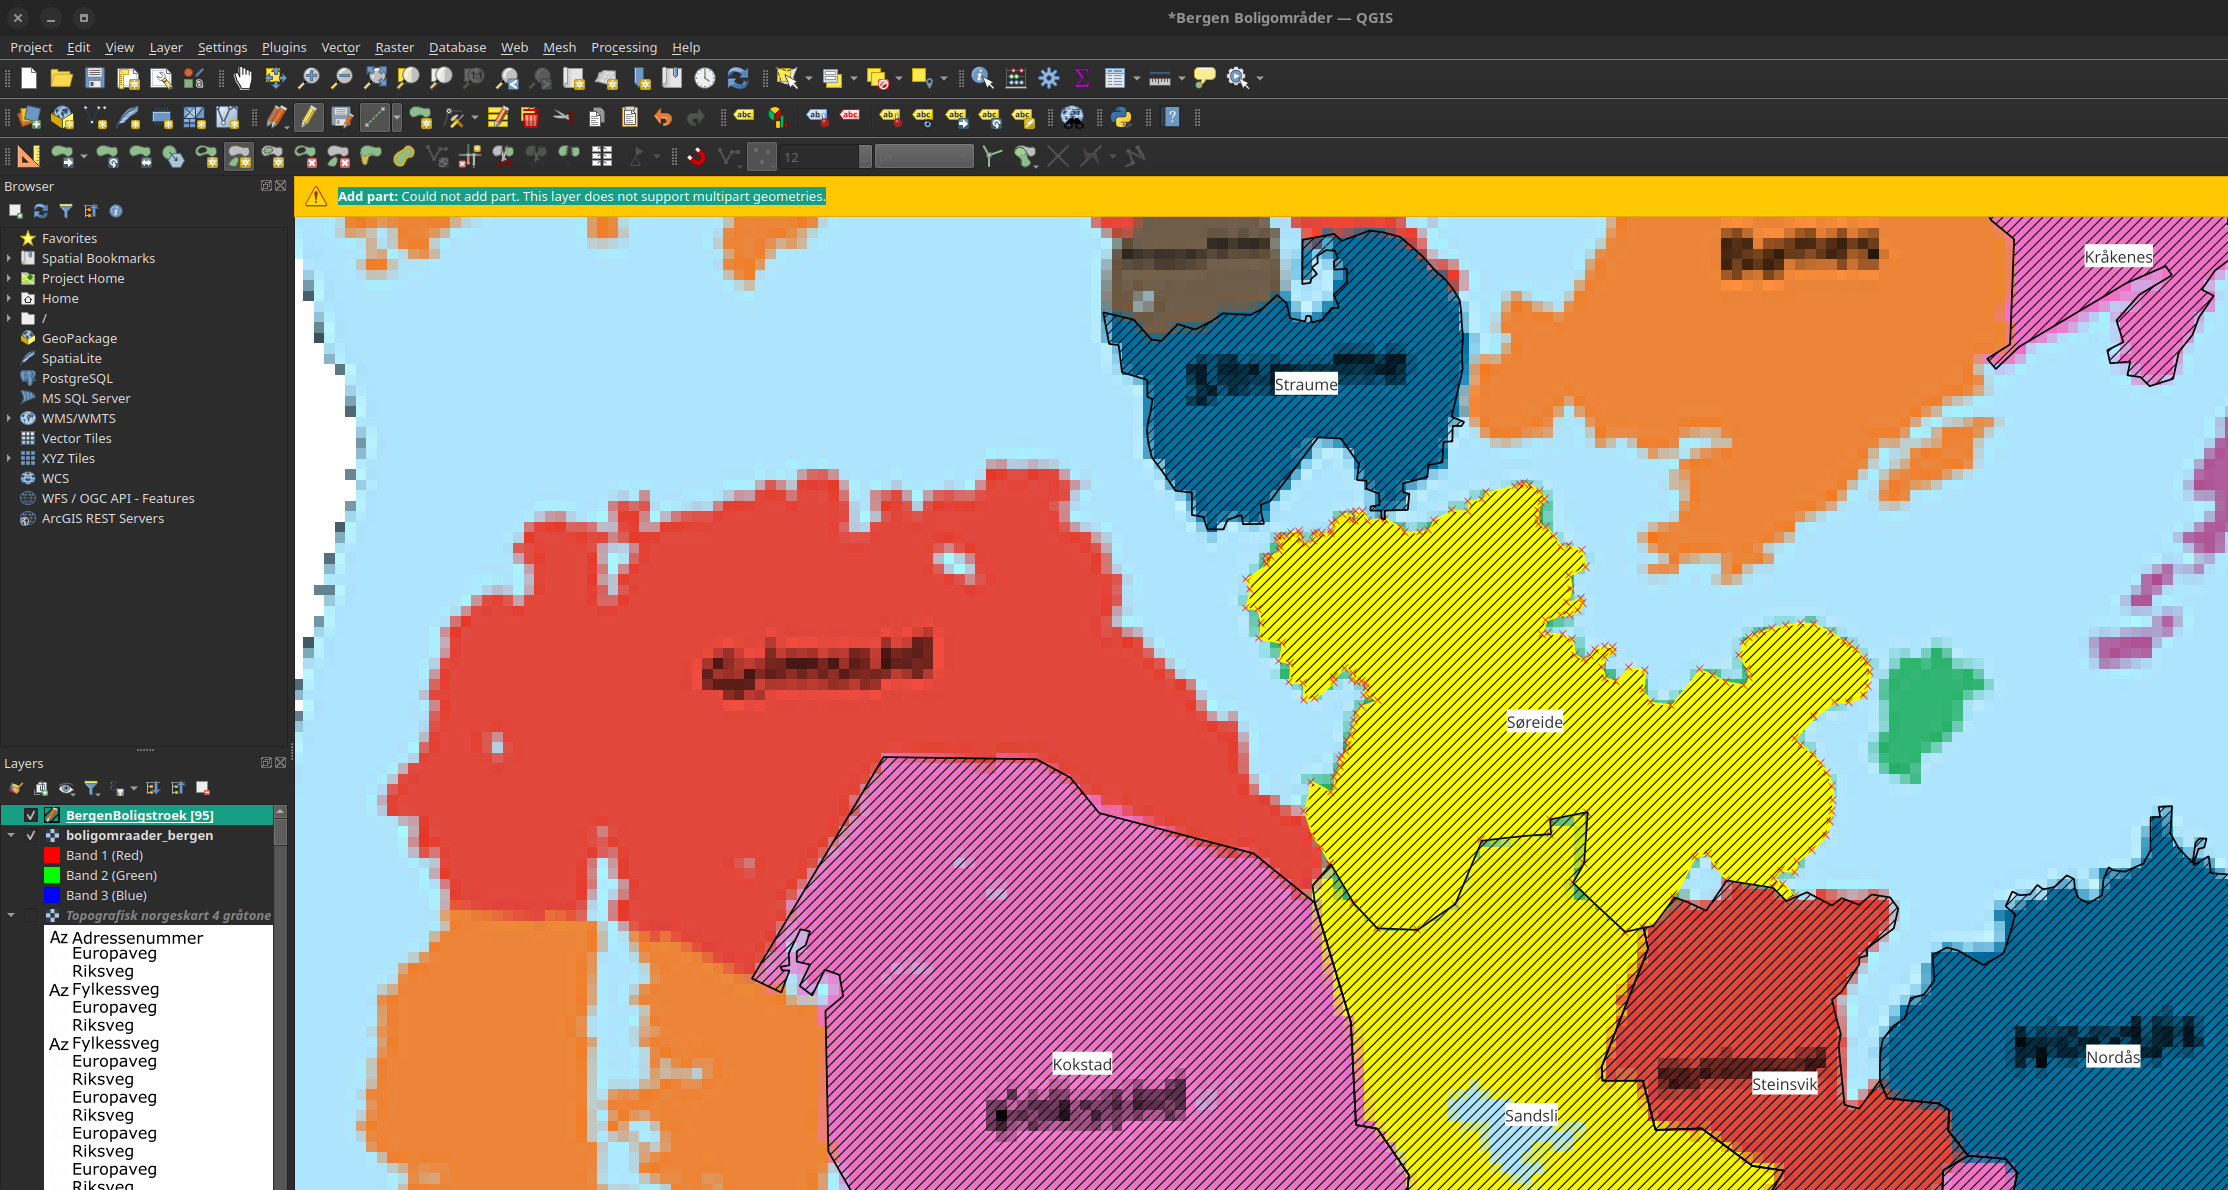
\includegraphics[height = 6cm]{images/qgis_multipart.png}%
%        \caption{}
%    \end{figure}
\end{frame}

% ====================================
\subsection{Export}
\begin{frame}
    \begin{figure}
        \centering
        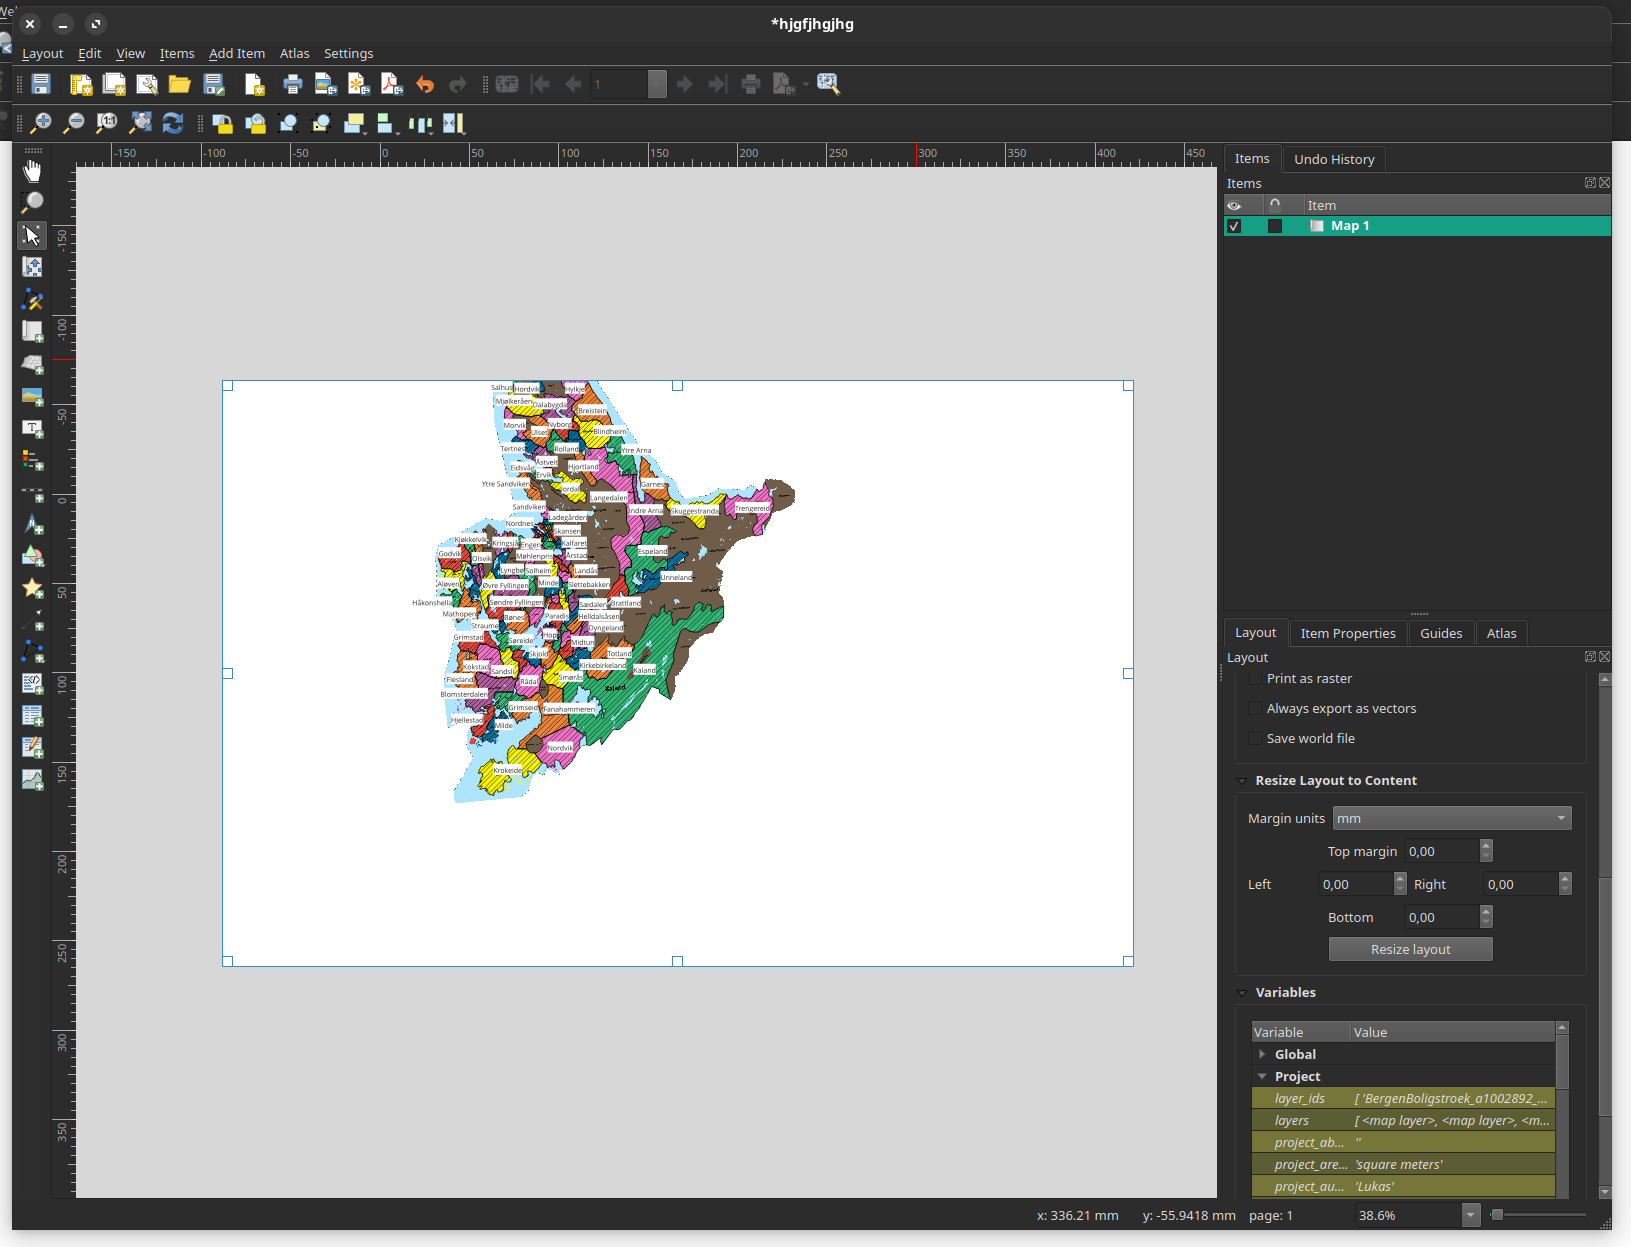
\includegraphics[height = 6cm]{images/qgis_export.png}%
        \caption{Ka e det?}
    \end{figure}
\end{frame}

\begin{frame}
    \begin{block}{Stackoverflow}
        \enquote{You have to select \textit{Vector Data Management Tools Split Vector Layer} on page 4 of the print menu. This will give you one SVG for the entire area and then you can dismantle the SVG file.}
    \end{block}
\end{frame}



\begin{frame}
    \begin{figure}
        \centering
        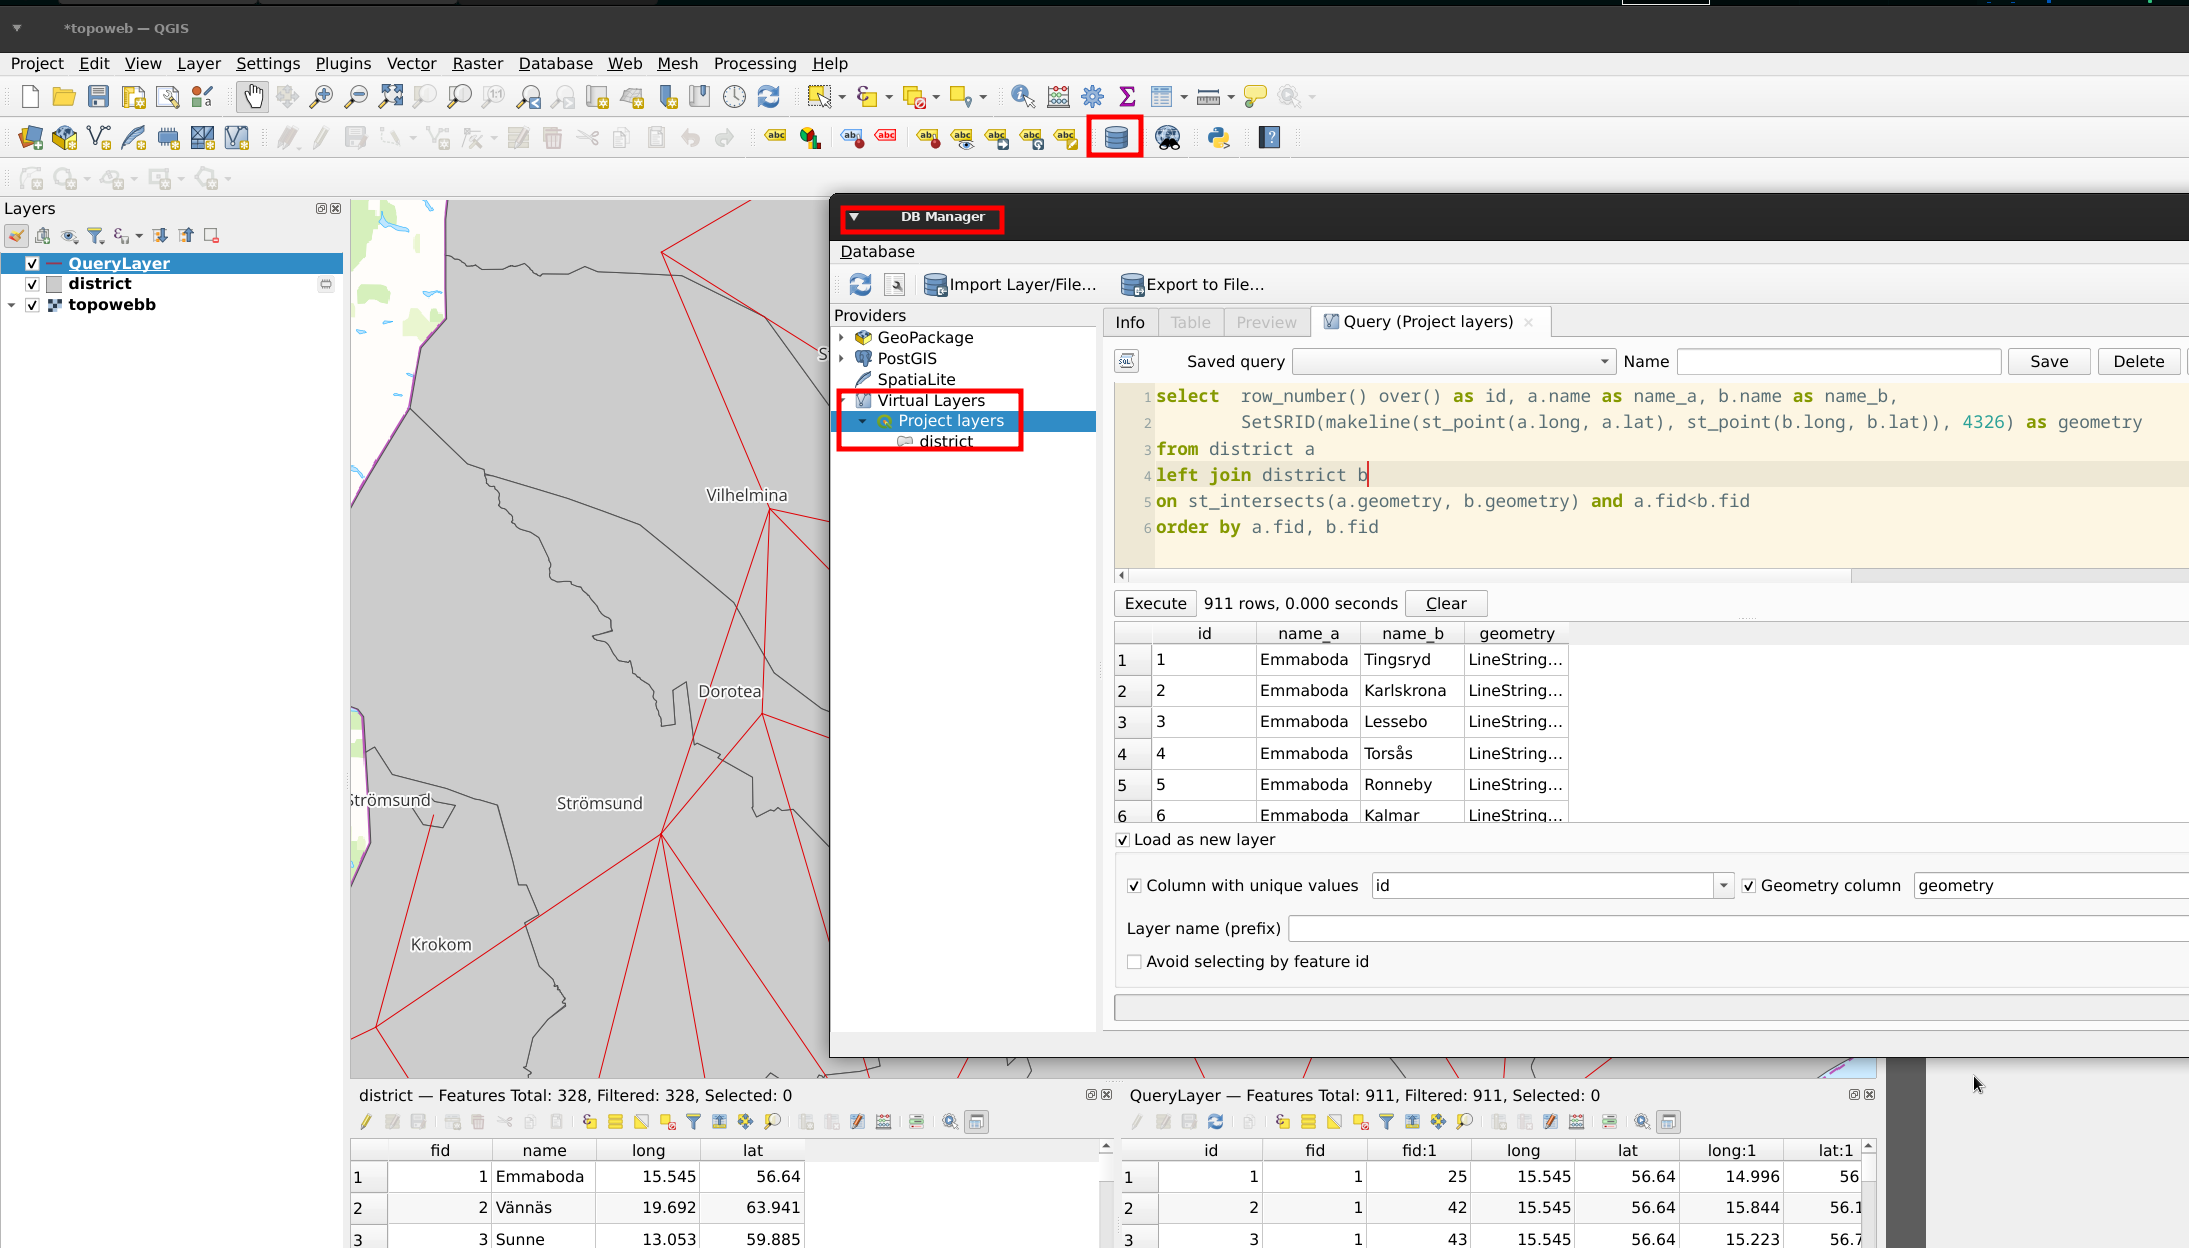
\includegraphics[height = 6cm]{images/qgis_sql.png}%
        \caption{Inline SQL}
    \end{figure}
\end{frame}

\begin{frame}
    \begin{figure}
        \centering
        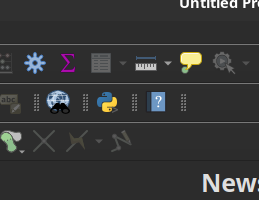
\includegraphics[height = 6cm]{images/qgis_python.png}%
        \caption{Insert Python?}
    \end{figure}
\end{frame}

\begin{frame}
    \begin{figure}
        \centering
        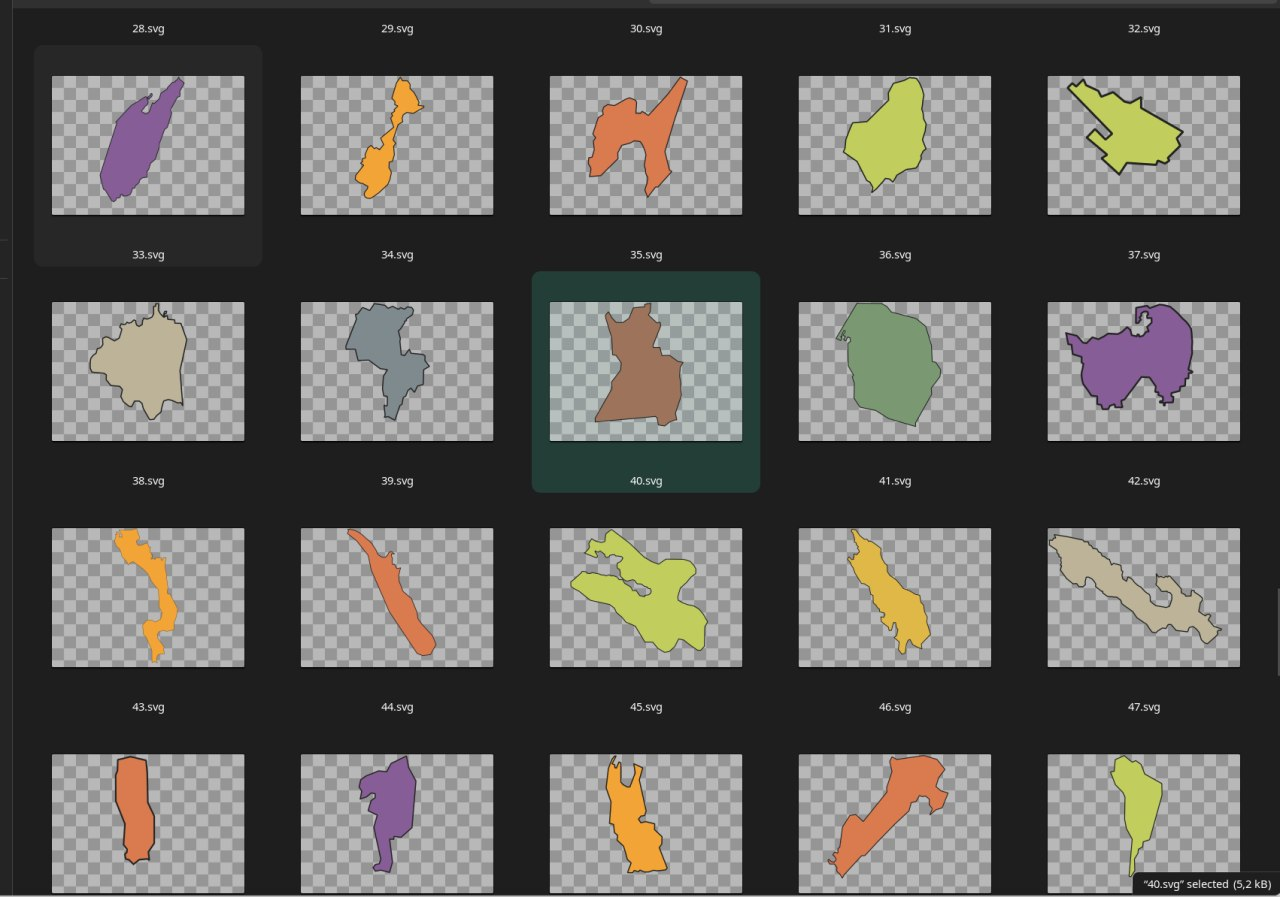
\includegraphics[height = 6cm]{images/svg_finished.jpg}%
        \caption{Ferdig!}
    \end{figure}
\end{frame}

\begin{frame}
    \begin{figure}
        \centering
        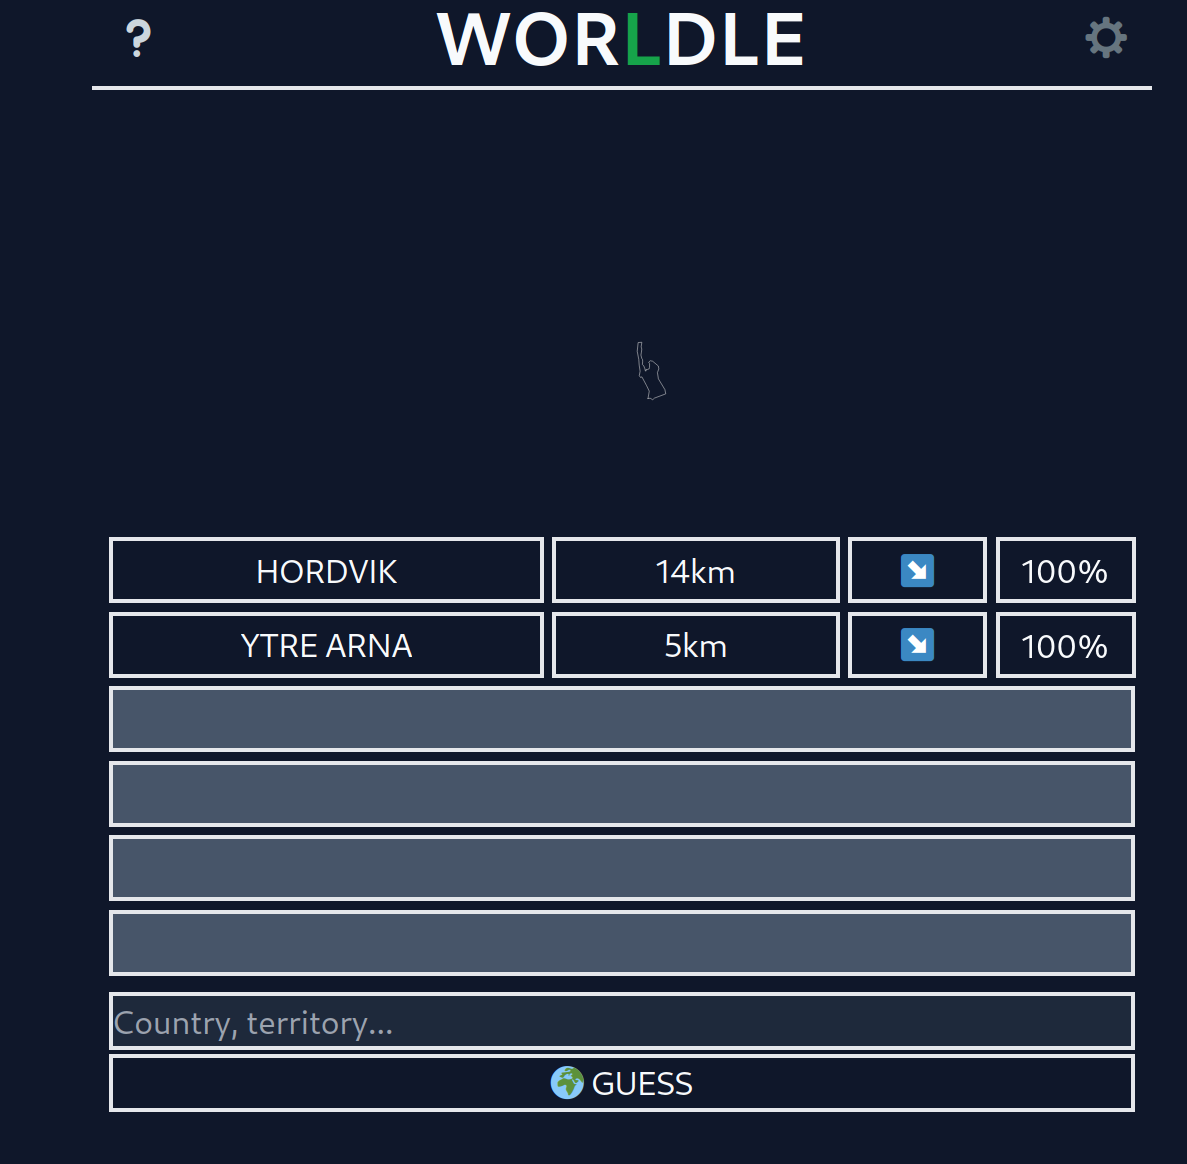
\includegraphics[height = 6cm]{images/svg_toosmall.png}%
        \caption{Enda mer fikling trengs}
    \end{figure}
\end{frame}